
\subsection{Reševanje}

Ponovno pripravim matriko, ki v diskretni obliki opisuje operator $\nabla^2$. Tokrat ni simetrična, zato sem pri uporabi \texttt{scipy.sparse.linalg} našel kompleksne rešitve (sicer z imaginarno komponento, primerljivo z $\varepsilon_\text{machine}$). S knjižnjico \texttt{scipy.linalg} teh problemov nisem imel, zato sem se posluževal slednje. Na podlagi rezultatov prve naloge pričakujem, da bi se metodi dobro ujemali in bo nadaljnje obnašanje rešitev podobno.

Ko sem lastne vektorje in vrednosti izračunal, sem si jih izrisal v polarni geometriji.

\begin{center}
    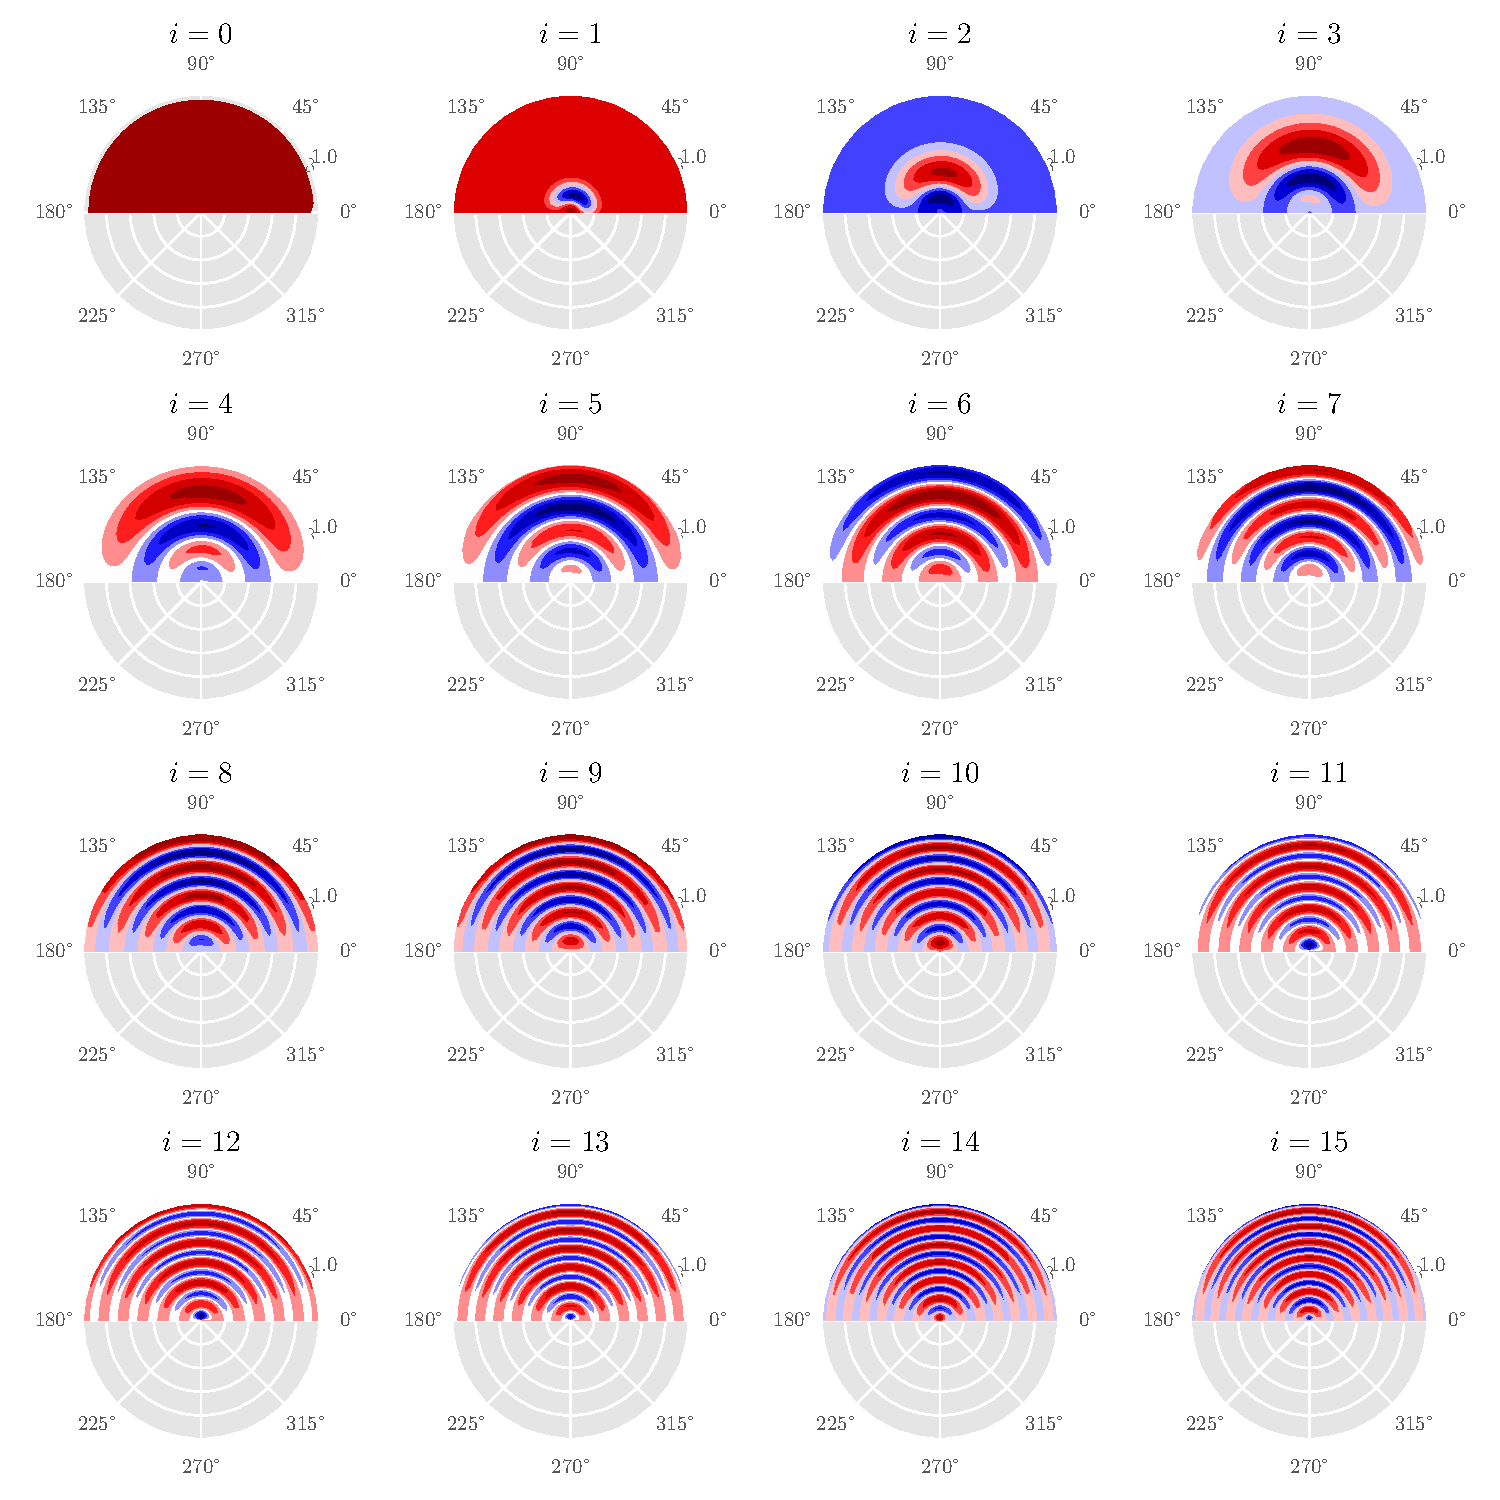
\includegraphics[width=0.9\textwidth]{../old/2-nihajni_nacini.pdf}
\end{center}
Ker me je skrbelo, zakaj  ne vidim večje polarne odvisnosti, sem pogledal tudi višje lastne nihajne načine in se uveril, da dobim pričakovano obnašanje tudi po polarnem kotu.



\begin{center}
    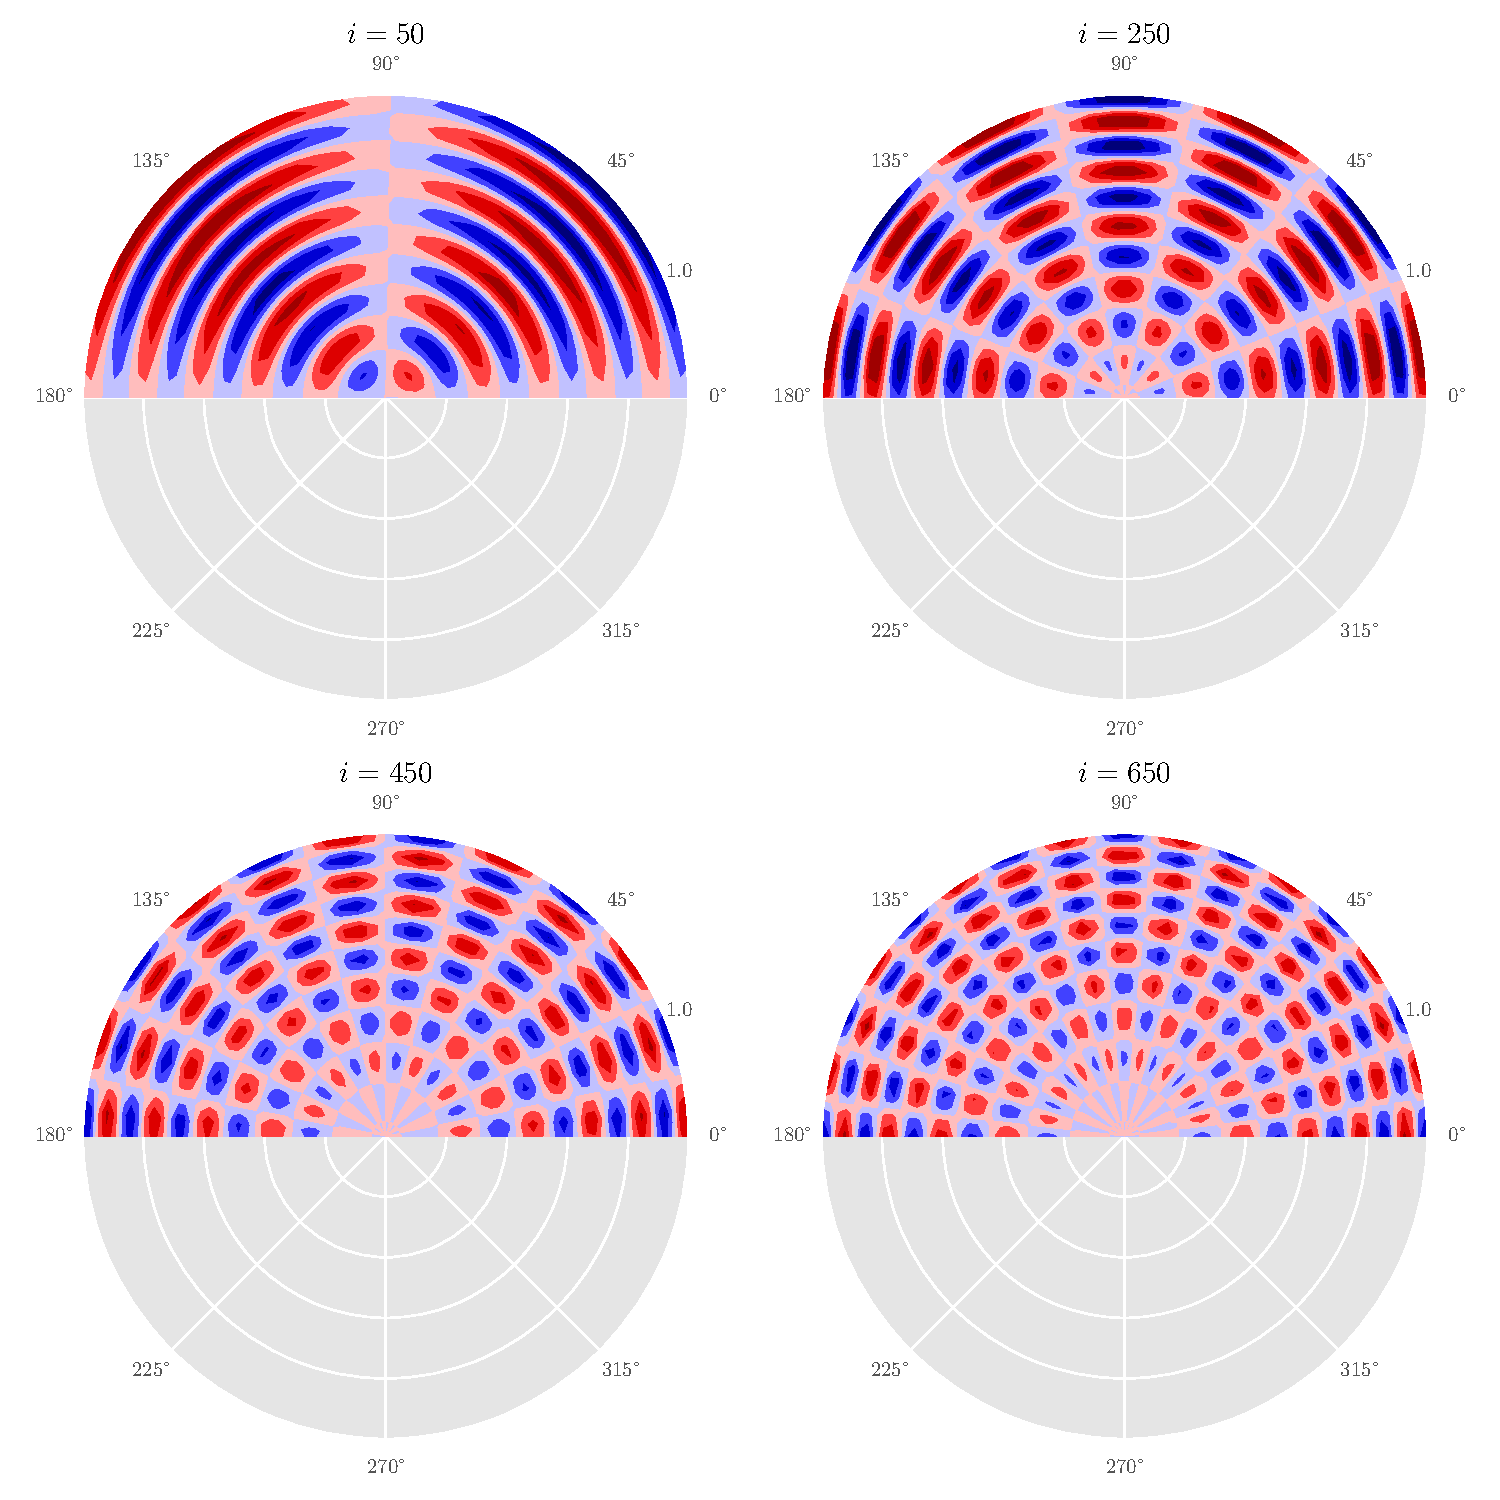
\includegraphics[width=0.8\textwidth]{../old/2-nihajni_nacini_miks.pdf}
\end{center}
Dobljen spekter lastnih vrednosti prikazujem spodaj.
\begin{center}
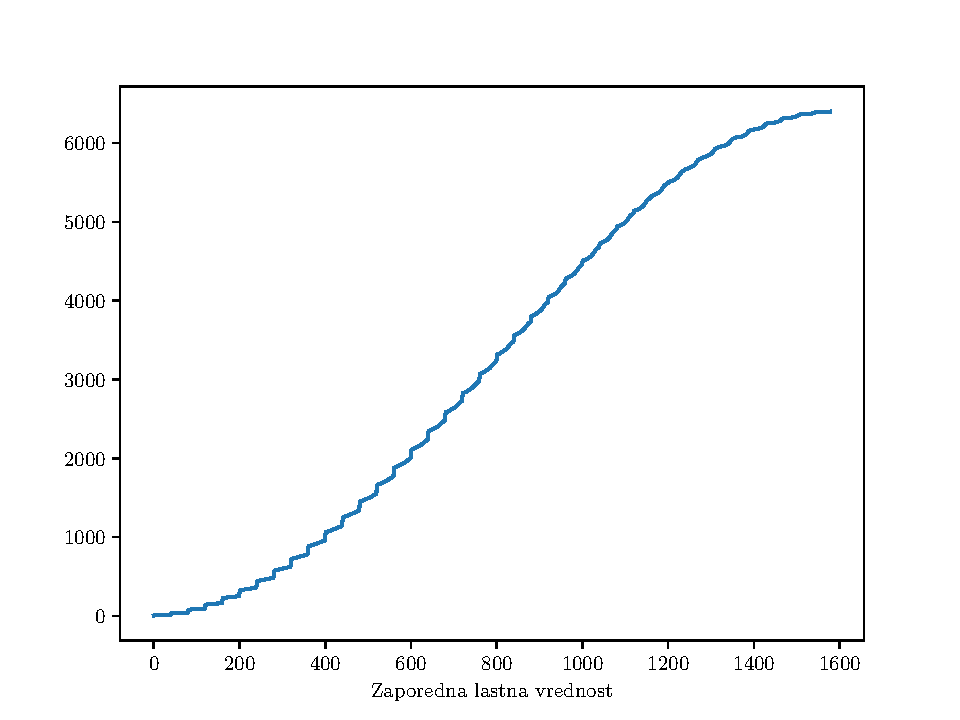
\includegraphics[width=0.7\textwidth]{../old/2-spekter.pdf}
\end{center}


\begin{thebibliography}{9}
\bibitem{wiki} \url{https://en.wikipedia.org/wiki/Inverse_iteration}

\end{thebibliography}
\end{document}

\begin{figure}
    \centering
        \begin{minipage}{0.45\textwidth}
        \centering
    \includegraphics[width=\textwidth]{../old/}
    \caption{}
        \label{fig:}
    \end{minipage}\hfill
    \begin{minipage}{0.45\textwidth}
        \centering
        \includegraphics[width=1\textwidth]{../old/}
    \caption{}
    \label{fig:}
    \end{minipage}
\end{figure}
